

\chapter{Förster Resonant Energy Transfer -- FRET}



\section{Experiment}

\textit{spektral, fl. Lifetime, ensemble, JK dyade
}
\textit{Wie groß ist der Förster-Radius des Paares? Wie groß ist die Transfer-Effizient in dieser Dyade?
}


\section{Forester Theory (FRET)\protect\footnote{Parson, ch. 7.2, Simon Biberger}} 


One way for an excited molecule to reach the ground state is by transferring this energy to another molecule. This is called resonance energy transfer.
At the beginning, two adjacent but non-interacting molecules 1 and 2 shall be considered. Their Hamiltonian operator is then
\begin{equation*}
    H = H_1 + H_2
\end{equation*}
and the associated overall wave function for the ground state is the product of the two individual wave functions.
\begin{equation*}
    \Psi_{Ges} = \Phi_{1a} \chi_{1a}\cdot \Phi_{2a} \chi_{2a}
\end{equation*}
If now one of the two molecules is excited, the total wave function becomes closed:
\begin{equation*}
    \Psi_{Ges} = C_1 \Phi_{1b} \chi_{1b}\cdot \Phi_{2a} \chi_{2a} + C_2 \Phi_{1a} \chi_{1a}\cdot \Phi_{2b} \chi_{2b}
\end{equation*}

The factors $C_1$ and $C_2$ represent the probability that the molecule is excited. Here $|C_1|^2 + |C_2|^2 = 1$.
In Förster theory, an interaction between the molecules is now allowed and the Hamilton operator is
\begin{equation*}
    H_{Ges} = H_1 + H_2 + H_{21}
\end{equation*}
If one starts at the time t\,=\,0 with $C_1$\,=\,1 and $C_2$\,=\,0, $C_2$ can be determined via time-dependent perturbation theory:
\begin{equation}
    C_2 = H_{21} \frac{1 - exp \left[\frac{i(E_2 - E_1)t}{\hbar} \right] } {E_2 - E_1}
    \label{c2}
\end{equation}
From equation \ref{c2} the resonance condition for the energy difference between molecule 1 and 2 can be derived immediately. $C_2$ has only a significant amount if the energy difference is as small as possible.


\begin{figure}
\label{Resonance}
\center
    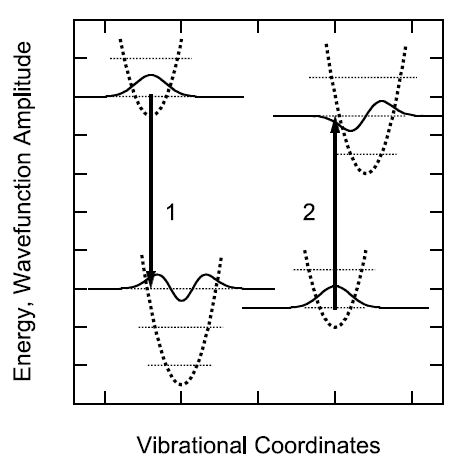
\includegraphics[width = 0.7 \textwidth]{\currfiledir/FRET.JPG}
    \caption{The resonance-energy transfer requires coupled vibronic transitions up and down. The energy lost by molecule 1 must be absorbed by molecule 2, so that the energy is maintained overall. In addition, the associated Frank-Condon factors for the transitions must be non-zero.}
\end{figure}

The total rate of energy transfer can be determined using Fermi's Golden Rule:
\begin{equation*}
    k_{rt} = \frac{2\pi}{\hbar} \cdot \int_{-\infty}^{+\infty} |H_{21}|^2 \rho_{s2}(E_1) \rho_{s1}(E_1) dE_1,
\end{equation*}
where $\rho_{si}$ denotes the state densities of molecule 1 and 2

\section{FRET on single molecules for distance measurement\protect\footnote{Parson, sections 7.2 and 7.3}} 

The strong distance dependence of FRET is used to
the relative spatial position of marker fluorophores
for example in proteins.

The transfer of energy from one excited fluorophore to another can be described with the theory of Förster resonance energy transfer. The energy transfer takes place without radiation via a dipole-dipole interaction. The rate constant $k_{rt}$ for this transition is defined as follows:
\begin{equation}
    k_{rt}=\left( \frac{9000 ln(10)\kappa^2c^4\Phi}{128\pi^5n^4N_A\tau} \right) |R_{21}|^{-6}J ,
\end{equation}
where $\kappa$ is the orientation factor, $\Phi$ and $\tau$ the quantum yield and lifetime of the donor, $R_{21}$ the distance between donor and acceptor, and J is an overlap integral between the absorption and emission spectrum of the fluorophores involved. The orientation factor $\kappa$ indicates the orientation of the two interacting partners assumed to be dipoles and can take values between $-2$ and $2$ (see Fig. \ref{KappaFactor}). 

\begin{figure}
\label{KappaFaktor}
\center
    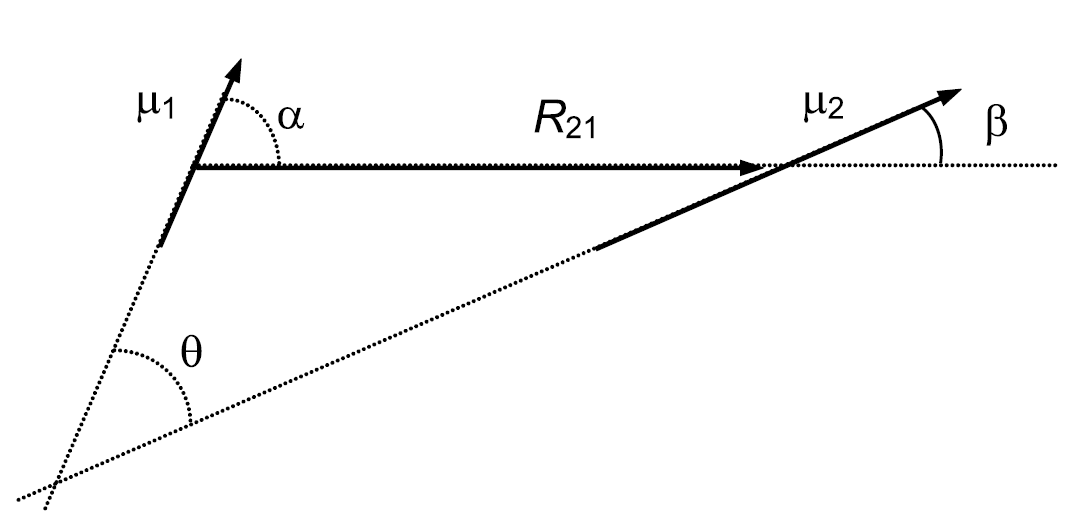
\includegraphics[width = 0.5 \textwidth]{\currfiledir/FretKappa.png}
    \caption{Sketch for the position of the angles and the distance of the dipoles. The orientation factor $\kappa$ is described by: $\kappa=\cos(\theta)-3 \cos (\alpha)\cos (\beta)$}
\end{figure}
The equation for the rate constant is also often given in the shortened form
\begin{equation}
\label{eq:fret}
    k_{rt}=\tau^{-1}(|R_{21}|/R_0)^{-6}
\end{equation}
with the forest ranger radius $R_0$. This indicates the distance at which the efficiency\footnote{The efficiency $E$ is defined as $E=\frac{1}{1+(r/R_0)^6}$ } of the energy transfer is 50\%.\par
To determine the distance between two molecules using Fret, the rate constant $k_{rt}$ must first be calculated from the fluorescence yields in the presence $\Phi$ and absence of the acceptor $\Phi_q$ using the following formula 
\[ \frac{\Phi}{\Phi_q}=1+k_{rt}\tau .\]
If the product of $k_{rt}\tau$ and the forester radius is known, the distance $|R_{21}|$ can be calculated from equation \ref{eq:fret}.




\printbibliography[segment=\therefsegment,heading=subbibliography]
